
\documentclass[border=10pt]{standalone}

\usepackage{tikz}
\usetikzlibrary{fit,positioning,calc}

\begin{document}

%default strings
\providecommand{\tstrcommunication}{Communication\\ protocol}
\providecommand{\tstrobjects}{Objects}
\providecommand{\tstrucode}{Microcode}
\providecommand{\tstrhbusstack}{HBUS Stack}
\providecommand{\tstrhbusdevice}{HBUS Device}
\providecommand{\tstrdevicecode}{Device code (firmware)}

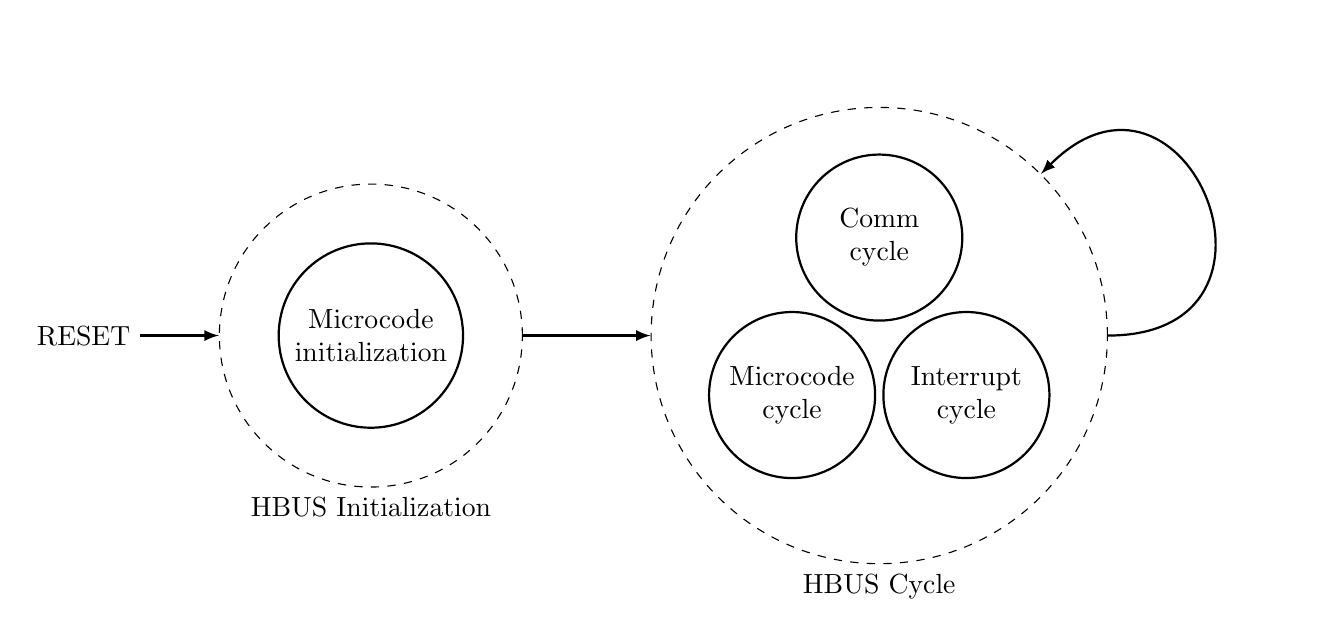
\begin{tikzpicture}[auto]

\tikzstyle{stackitem}=[rounded corners,thick,circle,minimum size=60pt,draw=black, node distance=5pt]

%init
\node [stackitem,align=center] (ucode) {Microcode \\ initialization};
\node [dashed,circle,fit= (ucode),inner sep=5pt,draw=black,label=270:{HBUS Initialization}] (hbusinit) {};


%reset
\node [left = of hbusinit] (reset) {RESET};

\path [-latex,thick] (reset) edge (hbusinit);

%cycle

\node [stackitem,align=center,above = of ucode.east,xshift=150pt] (comm) {Comm \\ cycle};
\node [stackitem,align=center,below = of comm.south west,xshift=-10pt] (ucodecycle) {Microcode \\ cycle};
\node [stackitem,align=center,below = of comm.south east,xshift=10pt] (intcycle) {Interrupt \\ cycle};

\node[dashed,draw=black,circle,fit=(comm) (ucodecycle) (intcycle),label=270:{HBUS Cycle},inner sep=-2pt] (hbuscycle) at (ucode -| comm) {};

\path [-latex,thick] (hbuscycle) edge [out=0,in=45,looseness=3] (hbuscycle)
      [-latex,thick] (hbusinit)  edge (hbuscycle);


\end{tikzpicture}
\end{document}